% !TEX root = ../probability_hse_exams.tex

\newpage
\thispagestyle{empty}
\section{Контрольная работа 1}


% \subsection[что идет в оглавление]{\hyperref[на что ссылка]{текст ссылки}}
\subsection[2018-2019]{\hyperref[sec:sol_kr_01_2018_2019]{2018-2019}}
\label{sec:kr_01_2018_2019} % \label{ссылка сюда}

На минимум в 4 вопроса было выделено 30 минут, на основную часть — 80 минут.

\begin{enumerate}

    %Задача 1
    \item Вася пришел на экзамен, зная всего 2 билета из 25. Каждый студент достает ровно один билет. Билеты, вытянутые студентами, обратно не возвращаются. Вася не знает, какие билеты попались другим студентам. Найдите вероятность того, что Вася достанет известный билет, если он будет тянуть билет:

    \begin{enumerate}
		\item вторым по счету (2 балла)
        \item двадцатым по счету (2 балла)
        \item двадцать пятым по счету (2 балла)
     \end{enumerate}

     \textbf{Ответ обоснуйте математически!}

    %Задача 2
    \item Игральный кубик с шестью гранями подбрасывается один раз. Рассмотрим две случайные величины:
    \begin{center}
    $\xi=\begin{cases}1\text{, если выпала единица}\\0\text{, в противном случае}\end{cases}$

    $\eta=\begin{cases}1\text{, если выпала шестерка}\\0\text{, в противном случае}\end{cases}$

    \begin{enumerate}
		\item Составьте таблицу совместного распределения случайных величин $\xi$ и $\eta$ (3 балла)
		\item Являются ли случайные величины $\xi$ и $\eta$ независимыми? Обоснуйте свой ответ! (1 балл)
		\item Найдите функцию распределения случайной величины $\xi+\eta$ и постройте её график (3 балла)
		\item Найдите распределение случайной величины $\xi$, при условии, что $\xi+\eta=1$ (3 балла)
     \end{enumerate}
     \end{center}
     %Задача 3
    \item Плотность распределения случайной величины $\xi$ имеет вид:

    \begin{center}
    $f_{\xi}(X)=\begin{cases}cx^2\text{, при }x\in[0,1]\\ 0\hspace{0.33cm}\text{, при }x\notin[0,1]\space\end{cases}$
    \end{center}

    Найдите

    \begin{enumerate}
		\item константу $c$ (2 балла)
		\item $\P(\xi=\frac{1}{2})$ и $P(\xi\in[0,\frac{1}{3}])$ (2 балла)
		\item функцию распределения случайной величины $\xi$ (2 балла)
		\item $\P(\xi\in[\frac{1}{3},\frac{3}{2}])$ (3 балла)
		\item $\P(\xi\leq\frac{1}{2}|\xi\geq\frac{1}{3})$ (2 балла)
		\item моду, медиану и математическое ожидание случайной величины $\xi$ (6 баллов)
     \end{enumerate}

	%Задача 4
    \item Вероятность того, что подсудимый действительно виновен равна p.
    Своё решение о подсудимом (виновен или невиновен) независимо друг от друга выносят 12 присяжных.
    Каждый присяжный выносит верное решение (за обвинение, если подсудимый виновен, и за оправдание, если подсудимый невиновен) с вероятностью 2/3.

    Найдите

    \begin{enumerate}
		\item наиболее вероятное число правильно проголосовавших присяжных (2 балла)
        \item вероятность того, что правильно проголосуют ровно $7$ присяжных (1 балл)
        \item вероятность вынесения обвинительного приговора ровно семью присяжными как функцию от параметра $p$ (4 балла)
        \item параметр $p$, если вероятность в пункте в) равна 0.17 (10 баллов)
     \end{enumerate}

     %Задача 5
     \item В лифт $12$-этажного дома на первом этаже вошли $11$ человек. Каждый из них выходит независимо от других и с равной вероятностью на любом из этажей, начиная со второго. Найдите вероятность того, что

     \begin{enumerate}
		\item поднимаясь вверх, на каждом этаже со второго по $12$-й будет выходит ровно один человек (5 баллов)
		\item все пассажиры выйдут не выше $9$-го этажа, если никто из них не вышел на первых пяти этажах (5 баллов)
     \end{enumerate}

\end{enumerate}


\newpage
% \subsection[что идет в оглавление]{\hyperref[на что ссылка]{текст ссылки}}
\subsection[2017-2018]{\hyperref[sec:sol_kr_01_2017_2018]{2017-2018}}
\label{sec:kr_01_2017_2018} % \label{ссылка сюда}

% * — не идёт в оглавление
\subsubsection*{Минимум}

\begin{enumerate}
\item Функция распределения случайной величины: определения и свойства.
\item Экспоненциальное распределение: определение, математическое ожидание и дисперсия.
\item В операционном отделе банка работает 80\% опытных сотрудников и 20\% неопытных. Вероятность совершения ошибки при очередной банковской операции опытным сотрудником равна $0.01$, а неопытным — $0.1$. Известно, что при очередной банковской операции была допущена ошибка. Найдите вероятность того, что ошибку допустил неопытный сотрудник.
\item При работе некоторого устройства время от времени возникают сбои. Количество сбоев за сутки имеет распределение Пуассона. Среднее количество сбоев за сутки равно 3. Найдите вероятность того, что за двое суток не произойдет ни одного сбоя.

\end{enumerate}

\subsubsection*{Задачи}

\begin{enumerate}

\item Правильный кубик подбрасывают один раз. Событие $A$ — выпало чётное число, событие $B$ — выпало число кратное трём, событие $C$ — выпало число, большее трёх.

\begin{enumerate}
\item Сформулируйте определение независимости двух событий;
\item Определите, какие из пар событий $A$, $B$ и $C$ будут независимыми.
\end{enumerate}


\item Теоретический минимум (ТМ) состоит из 10 вопросов, задачный (ЗМ) — из 24 задач.
Каждый вариант контрольной содержит два вопроса из ТМ и две задачи из ЗМ.
Чтобы получить за контрольную работу оценку 4 и выше, необходимо и достаточно правильно ответить на каждый вопрос ТМ и задачу ЗМ доставшегося варианта. Студент Вася принципиально выучил только $k$ вопросов ТМ и две трети ЗМ.
\begin{enumerate}
\item Сколько всего можно составить вариантов, отличающихся хотя бы одним заданием в ТМ или ЗМ части? Порядок заданий внутри варианта не важен.
\item Найдите вероятность того, что Вася правильно решит задачи ЗМ;
\item Дополнительно известно, что Васина вероятность правильно ответить на вопросы ТМ, составляет $1/15$. Сколько вопросов ТМ выучил Вася?
\end{enumerate}

\item Производитель молочных продуктов выпустил новый низкокалорийный йогурт Fit и утверждает, что он вкуснее его более калорийного аналога Fat.
Четырем независимым экспертам предлагают выбрать наиболее вкусный йогурт из трёх, предлагая им в одинаковых стаканчиках в случайном порядке два Fat и один Fit.
Предположим, что йогурты одинаково привлекательны.
Величина $\xi$ — число экспертов, отдавших предпочтение Fit.
\begin{enumerate}
\item Какова вероятность, что большинство экспертов выберут Fit?
\item Постройте функцию распределения величины $\xi$;
\item Каково наиболее вероятное число экспертов, отдавших предпочтение йогорту Fit?
\item Вычислите математическое ожидание и дисперсию $\xi$.
\end{enumerate}

\item Дядя Фёдор каждую субботу закупает в магазине продукты по списку, составленному котом Матроскином. Список не изменяется, и в него всегда входит 1 кг сметаны, цена которого является равномерно распределённой величиной $\alpha$, принимающей значения от 250 до 1000 рублей. Стоимость остальных продуктов из списка в тысячах рублей является случайной величиной $\xi$ с функцией распределения

\[
F(x)=\begin{cases}
1-\exp(-x^2 ), \text{ если } x \geq 0 \\
0, \text{ иначе.}\\
\end{cases}
\]

\begin{enumerate}
\item Какую сумму должен выделить кот Матроскин дяде Фёдору, чтобы её достоверно хватало на покупку сметаны?
\item Какую сумму должен выделить кот Матроскин дяде Фёдору, чтобы Дядя Фёдор с вероятностью 0.9 мог оплатить продукты без сметаны?
\item Найдите математическое ожидание стоимости продуктов без сметаны;
\item Найдите математическое ожидание стоимости всего списка.
\item Какова вероятность того, что общие расходы будут в точности равны их математическому ожиданию?
\end{enumerate}

Подсказка: $\int_0^{\infty} \exp(-x^2) \, dx = \sqrt{\pi} / 2$.

\item Эксперт с помощью детектора лжи пытается определить, говорит ли подозреваемый правду. Если подозреваемый говорит правду, то эксперт ошибочно выявляет ложь с вероятностью 0.1. Если подозреваемый обманывает, то эксперт выявляет ложь с вероятностью 0.95.

В деле об одиночном нападении подозревают десять человек, один из которых виновен и будет лгать, остальные невиновны и говорят правду.

\begin{enumerate}
\item Какова вероятность того, что детектор покажет, что конкретный подозреваемый лжёт?
\item Какова вероятность того, что конкретный подозреваемый невиновен, если детектор показал, что он лжёт?
\item Какова вероятность того, что эксперт верно выявит преступника,
то есть про каждого невиновного решит, что тот говорит правду, а про преступника решит, что
преступник лжёт?
\item Какова вероятность того, что эксперт ошибочно выявит  преступника, то есть покажет, что лжёт невиновный, а все остальные говорят правду?
\end{enumerate}
\end{enumerate}


\newpage
\subsection[2016-2017]{\hyperref[sec:sol_kr_01_2016_2017]{2016-2017}}
\label{sec:kr_01_2016_2017}

\begin{enumerate}
\item Из семей, имеющих двоих разновозрастных детей, случайным образом выбирается одна семья.
Известно, что в семье есть девочка (событие $A$).

\begin{enumerate}
\item	Какова вероятность того, что в семье есть мальчик (событие $B$)?
\item	Сформулируйте определение независимости событий и проверьте,
являются ли события $A$ и $B$ независимыми?
\end{enumerate}

\item Система состоит из $N$ независимых узлов.
При выходе из строя хотя бы одного узла, система дает сбой.
Вероятность выхода из строя любого из узлов равна $0.000001$.
Вычислите максимально возможное число узлов системы,
при котором вероятность её сбоя не превышает $0.01$.

\item Исследование состояния здоровья населения в шахтерском регионе
«Велико-кротовск» за пятилетний период показало,
что из всех людей с диагностированным заболеванием легких, 22\% работало на шахтах.
Из тех, у кого не было диагностировано заболевание легких, только 14\% работало на шахтах.
Заболевание легких было диагностировано у 4\% населения региона.

\begin{enumerate}
\item	Какой процент людей среди тех, кто работал в шахте,
составляют люди с диагностированным заболеванием легких?
\item	Какой процент людей среди тех, кто НЕ работал в шахте,
составляют люди с диагностированным заболеванием легких?
\end{enumerate}

\item  Студент Петя выполняет тест (множественного выбора) проставлением ответов наугад.
В тесте 17 вопросов, в каждом из которых пять вариантов ответов и только один из них правильный.
Оценка по десятибалльной шкале формируется следующим образом:
\[
\text{Оценка} =
\begin{cases}
\text{ЧПО} - 7, & \text{если $\text{ЧПО}\in [8;\,17]$,} \\
1,              & \text{если $\text{ЧПО}\in [0;\,7]$}
\end{cases}
\]
где ЧПО означает число правильных ответов.

\begin{enumerate}
\item	Найдите наиболее вероятное число правильных ответов.
\item	Найдите математическое ожидание и дисперсию числа правильных ответов.
\item	Найдите вероятность того, что Петя получит «отлично»
(по десятибалльной шкале получит 8, 9 или 10 баллов).

Студент Вася также выполняет тест проставлением ответов наугад.

\item	Найдите вероятность того, что все ответы Пети и Васи совпадут.
\end{enumerate}

\item  Продавец высокотехнологичного оборудования контактирует с одним или двумя
потенциальными покупателями в день с вероятностями $1/3$ и $2/3$ соответственно.
Каждый контакт заканчивается «ничем» с вероятностью $0.9$ и покупкой оборудования
на сумму в 50\,000 у.\,е. с вероятностью $0.1$.
Пусть $\xi$ — случайная величина, означающая объем дневных продаж в у.\,е.

\begin{enumerate}
\item	Вычислите  $\P(\xi = 0)$.
\item	Сформулируйте определение функции распределения и постройте функцию распределения
случайной величины $\xi$.
\item	Вычислите математическое ожидание и дисперсию случайной величины $\xi$.
\end{enumerate}

\item Интервал движения поездов метро фиксирован и равен $b$ минут,
т.е. каждый следующий поезд появляется после предыдущего ровно через $b$ минут.
Пассажир приходит на станцию в случайный момент времени.
Пусть случайная величина $\xi$, означающая время ожидания поезда,
имеет равномерное распределение на отрезке $[0; b]$.

\begin{enumerate}
\item Запишите плотность распределения случайной величины $\xi$.
\item	Найдите константу $b$, если известно, что в среднем пассажиру приходится
ждать поезда одну минуту, т.\,е. $\E(\xi) = 1$.
\item	Вычислите дисперсию случайной величины $\xi$.
\item	Найдите вероятность того, что пассажир будет ждать поезд менее одной минуты.
\item	Найдите квантиль порядка $0.25$ распределения случайной величины $\xi$.
\item	Найдите центральный момент порядка 2017 случайной величины $\xi$.
\item	Постройте функцию распределения случайной величины $\xi$.

Марья Ивановна из суеверия всегда пропускает два поезда и садится в третий.

\item	Найдите математическое ожидание и дисперсию времени,
затрачиваемого Марьей Ивановной на ожидание «своего» поезда.

Глафира Петровна не садится в поезд, если видит в нем подозрительного человека.
Подозрительные люди встречаются в каждом поезде с вероятностью $3/4$.

\item	Найдите вероятность того, что Глафире Петровне придется ждать не менее пяти минут,
чтобы уехать со станции.
\item	Найдите математическое ожидание времени ожидания «своего» поезда для Глафиры Петровны.
\end{enumerate}

\item (Бонусная задача)
На первом этаже десятиэтажного дома в лифт заходят 9 человек.
Найдите математическое ожидание числа остановок лифта, если люди выходят из лифта независимо друг от друга.
\end{enumerate}


\newpage
\subsection[2015-2016]{\hyperref[sec:sol_kr_01_2015_2016]{2015-2016}}
\label{sec:kr_01_2015_2016}

\begin{enumerate}
\item
Подбрасываются две симметричные монеты. Событие $А$ — на первой монете выпал
герб, событие $В$ — на второй монете выпал герб, событие $С$ — монеты выпали
разными сторонами.
\begin{enumerate}
    \item[$\alpha$)] Будут ли эти события попарно независимы?
    \item[$\beta$)]  Сформулируйте определение независимости в совокупности для трех событий. Являются ли события $A$, $B$, $C$ независимыми в совокупности?
\end{enumerate}

\item
Имеются два игральных кубика:
\begin{itemize}
    \item красный со смещенным центром тяжести, так что вероятность выпадения «6»
    равняется $1/3$, а оставшиеся грани имеют равные шансы на появление
    \item честный белый кубик
\end{itemize}

\begin{enumerate}
    \item[$\alpha$)] Петя случайным образом выбирает кубик и подбрасывает его.
    Найдите вероятность того, что выпадет «6».
    \item[$\beta$)]   Петя случайным образом выбирает кубик и подбрасывает его.
    Какова вероятность того, что Петя взял красный кубик, если известно, что выпала
    шестерка?
\end{enumerate}

\item
Все те же кубики. Петя играет с Васей в следующую игру: Петя выбирает кубик и
подбрасывает его. Вася подбрасывает оставшийся кубик. Выигрывает тот, у кого
выпало большее число. Если выпадает равное число очков, выигрывает тот, у кого
белый кубик.

Пусть случайная величина $\xi$ — число очков, выпавших на красном кубике,
случайная величина $\eta$ — число очков,
выпавших на белом кубике, а величина $\zeta$ — максимальное число очков.

\begin{enumerate}
    \item[$\alpha$)] Задайте в виде таблицы совместное распределение величин $\xi$ и $\eta$.
    Отметьте (* или кружочком) все те пары значений, когда выигрывает красный кубик.
    \item[$\beta$)] Какой кубик нужно выбрать Пете, чтобы его шансы выиграть были выше?
    \item[$\gamma$)] Сформулируйте определение функции распределения и постройте функцию
    распределения величины $\zeta$.
    \item[$\delta$)] Вычислите математическое ожидание величины $\zeta$.
\end{enumerate}

\item
Проводится исследование с целью определения процента мужчин, которые любят
петь в душе. Поскольку некоторые мужчины стесняются прямо отвечать на этот
вопрос, предлагается перед ответом на вопрос: «поете ли Вы, когда принимаете
душ?» подбросить правильный кубик, и выбрать ответ «ДА», если выпала
шестерка, ответ «НЕТ», если выпала единица, и честный ответ («ДА» или «НЕТ»),
если выпала любая другая цифра.

Предположим, что по результатам исследования
вероятность ответа «ДА» составляет $2/3$. Каков истинный процент «певцов»?

\item
Ваш полный тезка страдает дисграфией. При подписывании контрольной работы
по теории вероятностей в своих имени и фамилии в именительном падеже Ваш
тезка с вероятностью $0.1$ вместо нужной буквы пишет любую другую (независимо
от предыдущих ошибок).

\begin{enumerate}
    \item[$\alpha$)] Найдите вероятность того, что он напишет свою фамилию правильно.
    \item[$\beta$)] Найдите вероятность того, что он сделает ровно 2 ошибки в своем имени.
    \item[$\gamma)$] Вычислите наиболее вероятное число допущенных тезкой ошибок.
    \item[$\delta$)] Найдите вероятность того, что при подписывании работы Ваш тезка
    допустит хотя бы одну ошибку.
\end{enumerate}

\item
Время (в часах), за которое студенты выполняют экзаменационное задание
является случайной величиной с функцией плотности

\[
f(y) =
\begin{cases}
cy^2 + y , & \mbox{if } 0 \le y \le 1 \\
0, & \mbox{else}
\end{cases}
\]

\begin{enumerate}
    \item[$\alpha$)] Найдите константу $c$.
    \item[$\beta$)]  Найдите функцию распределения и постройте её.
    \item[$\gamma)$] Вычислите вероятность того, что случайно выбранный студент
    закончит работу менее чем за полчаса.
    \item[$\delta$)] Найдите медиану распределения.
    \item[$\epsilon$)] Определите вероятность того, что студент, которому требуется
    по меньшей мере 15 минут для выполнения задания, справится с ним более, чем за 30 минут.
\end{enumerate}

\item
Вам известно, что на большом листе бумаги $1.5$ м $\times$ $1$ м нарисован слон. Вам завязали
глаза и выдали кисточку хвоста для слона. Вам нужно прилепить эту кисточку к
листу (рисунок Вы не видели). Вы подходите к листу и произвольно приклеиваете
кисточку
\begin{enumerate}
    \item[$\alpha$)] Какова вероятность того, что кисточка окажется на слоне,
    если площадь рисунка составляет $1$ м$^2$?
    \item[$\beta$)] Запишите вид функции совместной плотности для координат кисточки.
    \item[$\gamma)$] Запишите вид частных функций плотности для каждой из координат кисточки.
    \item[$\delta$)] Являются ли координаты кисточки независимыми случайными величинами?
    \item[$\epsilon$)] Запишите вид функции плотности суммы координат кисточки.
\end{enumerate}
\textit{Подсказка: слон не должен заслонить равномерного распределения.}

\begin{center}
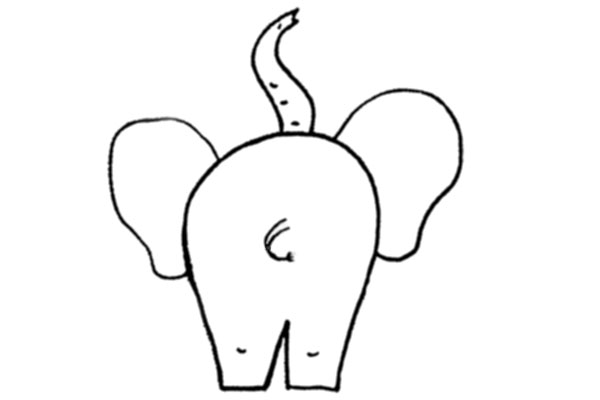
\includegraphics[scale=1.5]{images/slon.jpg}
\end{center}

\item
Укажите названия букв греческого алфавита и запишите соответствующие заглавные буквы:
\[\alpha, \zeta, \eta, \theta\].

\end{enumerate}



\newpage
\subsection[2014-2015]{\hyperref[sec:sol_kr_01_2014_2015]{2014-2015}}
\label{sec:kr_01_2014_2015}

\begin{enumerate}
\item Вася забыл какую-то (какую?) формулу. Он помнит, что она начинается
с «$\P(A|B) = $». Дальше была дробь, три буквы $\P$ со скобками после них и
в сумме по две буквы $A$ и $B$ внутри этих скобок. Ещё там была вертикальная черта «|».
Из этих элементов Вася случайным образом составляет формулу.
\begin{enumerate}
\item С какой вероятностью Вася напишет правильную формулу?
\item Напишите формулу, которую забыл Вася.
\end{enumerate}

Примечание: Вася всё-таки успел сходить на пару лекций по теории вероятностей и помнит,
что $\P(A|B)$ и $\P(B|A)$ — это не одно и то же, «|» должна стоять именно между буквами
(то ли $A|B$, то ли $B|A$), а в скобках, которые идут после $\P$, должно хоть что-то стоять.
При этом формула должна иметь смысл, то есть  $\P(A|B)$   не должна выражаться через себя же,
и дробь не должна быть сократимой.

\item Точка с координатами $(\xi, \eta)$ бросается наудачу в треугольник с вершинами
$(1,0)$, $(0,0)$, $(0,1)$. Сформулируйте определение независимости двух событий и
проверьте, будут ли события $A=\{ \xi < 1/2 \}$  и $B=\{ \eta < 1/2 \}$  независимыми?

\item На учениях три самолёта одновременно и независимо атакуют цель.
Известно, что первый самолёт поражает цель с вероятностью $0.6$, второй — $0.4$,
третий — $0.3$. При разборе учений выяснилось, что цель была поражена только
одним самолётом. Какова вероятность того, что это был первый самолёт?

\item Книга в $500$ страниц содержит $400$ опечаток. Предположим, что каждая
из них независимо от остальных опечаток может с одинаковой вероятностью оказаться
на любой странице книги.
\begin{enumerate}
\item Определите вероятность того, что на $13$-й странице будет не менее двух опечаток,
в явном виде и с помощью приближения Пуассона.
\item Определите наиболее вероятное число, математическое ожидание и дисперсию числа
опечаток на $13$-ой странице.
\item Является ли $13$-ая страница более «несчастливой», чем все остальные
(в том смысле, что на $13$-ой странице ожидается большее количество очепяток,
чем на любой другой)?
\end{enumerate}

Подсказка. Можно считать, что опечатки «выбирают» любую из страниц для своего
появления независимо друг от друга. Успех заключается в выборе $13$-ой страницы.
Вероятность успеха?

\item Вероятность того, что медицинский тест выявит наличие заболевания,
когда оно действительно есть, называется чувствительностью теста. Специфичностью
теста называется вероятность того, что тест покажет отсутствие заболевания,
когда пациент здоров. Вероятность того, что пациент болен, когда тест показал
наличие заболевания, называется прогностической силой теста. Предположим, что
только 1\,\%  всего населения страдает данным заболеванием.  Чувствительность
используемого теста равна $0.9$, а специфичность — $0.95$.
\begin{enumerate}
\item Какова вероятность того, что у случайно выбранного человека тест покажет
наличие заболевания?
\item Какова прогностическая сила теста? Что нужно сделать, чтобы её повысить?
\end{enumerate}

\item Функция плотности случайной величины $X$ имеет вид:
\begin{equation*}
f(x) =
 \begin{cases}
   1.5 (x-a)^2 &, x \in [0,a]\\
   1.5 (x+a)^2 &, x \in [-a,0]\\
   0 &, x \not\in [-a,a]
 \end{cases}
\end{equation*}

\begin{enumerate}
\item Найдите константу $a$, вероятность попадания в отрезок $\left[1/2, 2 \right]$,
математическое ожидание $X$ и дисперсию случайной величины $X$.
\item Нарисуйте функцию распределения случайной величины $X$.
\end{enumerate}

\item Вася случайным образом посещает лекции по ОВП (Очень Важному Предмету).
С вероятностью $0.9$ произвольно выбранная лекция полезна, и с вероятностью $0.7$ она интересна.
Полезность и интересность — независимые друг от друга и от номера лекции свойства.
Всего Вася прослушал 30 лекций.
\begin{enumerate}
\item Определите математическое ожидание и дисперсию числа полезных лекций и
числа интересных лекций, прослушанных Васей.
\item Определите математическое ожидание числа бесполезных и неинтересных лекций,
прослушанных Васей, и числа лекций, обладающих хотя бы одним из свойств (полезность,
интересность).
\end{enumerate}

\item Пусть $\E(X) = 1$, $\E(Y) = 2$, $\E\left(X^2\right) = 5$, $\E(XY) = -1$. Найдите:
\begin{enumerate}
\item $\E(2X + Y - 4)$
\item $\Var(X)$, $\Var(Y)$
\item $\Cov(X,Y)$, $\Corr(X,Y)$
\item $\Var(X-Y-1)$,  $\Var(X+Y+1)$
\item $\Cov(X-Y-1, X+Y+1)$,  $\Corr(X-Y-1, X+Y+1)$
\end{enumerate}

\item Совместное распределение случайных величин $X$ и $Y$ задано в виде таблицы:

\begin{center}
\begin{tabular}{ccc}
\toprule
 & $X=1$ & $X=2$ \\ \midrule
$Y=-1$ & $0.1$ & $0.2$ \\
$Y=0$ & $0.2$ & $0.3$ \\
$Y=1$ & $0$ & $0.2$ \\ \bottomrule
\end{tabular}
\end{center}

\begin{enumerate}
\item Найти частные распределения $Y$ и $Y^2$
\item Найти ковариацию случайных величин $X$ и $Y$
\item Можно ли утверждать, что случайные величины зависимы?
\end{enumerate}

\item Бонусная задача

Какова вероятность того, что наугад выбранный ответ на этот вопрос окажется верным
(искомую вероятность вычислить и записать!)?
\begin{enumerate}
\item 0.25
\item 0.5
\item 0.6
\item 0.25
\end{enumerate}
\end{enumerate}



\newpage
\subsection[2013-2014]{\hyperref[sec:sol_kr_01_2013_2014]{2013-2014}}
\label{sec:kr_01_2013_2014}


\begin{enumerate}
\item Вероятность застать Васю на лекции зависит от того, пришли ли на лекцию Маша и Алена.
Данная вероятность равна $0.18$, если девушек нет; $0.9$ — если обе девушки пришли на лекцию;
$0.54$ — если пришла только Маша и $0.36$ — если пришла только Алена.
Маша и Алена посещают лекции независимо друг от друга с вероятностями $0.4$ и $0.6$ соответственно.
\begin{enumerate}
\item Определите вероятность того, что на лекции присутствует Алена, если в аудитории есть Вася.
\item Кого чаще можно застать на тех лекциях, на которых присутствует Вася: Машу или Алену?
%\item При каком значении $p$ Вася посещает половину всех лекций?
\end{enumerate}

\item Страховая компания страхует туристов, выезжающих за границу,
от невыезда и наступления страхового медицинского случая за границей.
Застраховано 100 туристов. Вероятность «невыезда» за границу случайно
выбранного туриста — $0.002$, а страховые выплаты в этом случае — 2000 у.е.;
вероятность обращения за медицинской помощью за границей — $0.01$,
а страховые выплаты — 3000 у.е. Для каждого туриста рассмотрим две случайные
величины: $X_i$, равную 1 при невыезде за границу и 0 иначе, и $Y_i$, равную 1
при обращении за медицинской помощью и нулю иначе.
Обозначим $X=\sum_{i=1}^{100}X_i$ и $Y=\sum_{i=1}^{100}Y_i$.
\begin{enumerate}
\item Определите $\P(X=5)$, $\E(X)$, $\Var(X)$.
\item Наиболее вероятное число не выехавших туристов.
\item Вычислите математическое ожидание и дисперсию величины совокупных страховых выплат.
\end{enumerate}
Подсказка: Число обращений в страховую компанию для каждого туриста может быть
записано в виде $X_i+X_i Y_i$, так как медицинский страховой случай может наступить
только, если турист выехал за границу. Случайные величины $X_i$ и $Y_i$ независимы.

\item Функция плотности случайной величины $X$ имеет вид:
\begin{equation}
f(x)=\begin{cases}
ce^{-x}, \, x\geq 0 \\
ce^x, \, x<0
\end{cases}
\end{equation}
\begin{enumerate}
\item Найдите $c$, $\P(X \in [\ln 0.5,\ln 4])$, $\E(X)$, $\Var(X)$
\item Моменты всех порядков случайной величины $x$
\end{enumerate}

Подсказка: $\int_0^{\infty} x^n e^{-x} \, dx=n!$

\item Известно, что  $\E(X)=-1$, $\E(Y)=1$, $\Var(X)=9$, $\Var(Y)=4$, $\Corr(X,Y)=1$.
Найдите
\begin{enumerate}
\item $\E(Y-2X-3)$, $\Var(Y-2X-3)$
\item  $\Corr(Y-2X-3,X)$
\item Можно ли выразить $Y$ через $X$? Если да, то запишите уравнение связи.
\end{enumerate}

\item Совместное распределение доходов акций двух компаний $Y$ и $X$ задано в виде таблицы

\begin{center}
\begin{tabular}{@{}cccc@{}}
\toprule
    & $X=-1$ & $X=0$ & $X=1$ \\ \midrule
$Y=-1$ & $0.1$  & $0.2$   & $0.2$ \\
$Y=1$ & $0.2$  & $0.1$ & $0.2$ \\ \bottomrule
\end{tabular}
\end{center}

\begin{enumerate}
\item Найдите  частные распределения случайных величин $X$ и $Y$
\item Найдите $\Cov(X,Y)$
\item Можно ли утверждать, что случайные величины $X$ и $Y$ зависимы?
\item Найдите условное распределение случайной величины $X$ при условии $Y=-1$
\item Найдите условное математическое ожидание $\E(X\mid Y=-1)$
\end{enumerate}
\end{enumerate}



\newpage
\subsection[2012-2013]{\hyperref[sec:sol_kr_01_2012_2013]{2012-2013}}
\label{sec:kr_01_2012_2013}


\begin{enumerate}

\item Погода завтра может быть ясной с вероятностью $0.3$ и пасмурной с вероятностью $0.7$.
Вне зависимости от того, какая будет погода, Маша даёт верный прогноз с вероятностью $0.8$.
Вовочка, не разбираясь в погоде, делает свой прогноз по принципу: с вероятностью $0.9$
копирует Машин прогноз, и с вероятностью $0.1$ меняет его на противоположный.
\begin{enumerate}
\item Какова вероятность того, что Маша спрогнозирует ясный день?
\item Какова вероятность того, что Машин и Вовочкин прогнозы совпадут?
\item Какова вероятность того, что день будет ясный, если Маша спрогнозировала ясный?
\item Какова вероятность того, что день будет ясный, если Вовочка спрогнозировал ясный?
\end{enumerate}

\item Машин результат за контрольную, $M$, равномерно распределен на отрезке $[0;1]$.
Вовочка ничего не знает, поэтому списывает у Маши, да ещё может наделать ошибок при
списывании. Поэтому Вовочкин результат, $V$, распределен равномерно от нуля до Машиного
результата.
\begin{enumerate}
\item Найдите $\P(M>2V)$, $\P(M>V+0.1)$
\item Зачёт получают те, чей результат больше $0.4$. Какова вероятность того, что Вовочка получит зачёт? Какова вероятность того, что Вовочка получит зачёт, если Маша получила зачёт?
\end{enumerate}
Подсказка: попробуйте нарисовать нужные события в осях $(V,M)$

Это была задачка-неберучка!

\item Функция плотности случайной величины $X$ имеет вид
\[
f(x)=
\begin{cases}
\frac{3}{7}x^2, & x\in[1;2] \\
0,& x \notin [1,2]
\end{cases}
\]
\begin{enumerate}
\item Не производя вычислений найдите $\int_{-\infty}^{+\infty}f(x)\,dx$
\item Найдите $\E(X)$, $\E(X^2)$ и дисперсию $\Var(X)$
\item Найдите $\P(X>1.5)$
\item Найдите функцию распределения $F(x)$ и постройте её график
\end{enumerate}

\item Совместное распределение случайных величин $X$ и $Y$ задано таблицей

\begin{center}
\begin{tabular}{@{}cccc@{}}
\toprule
      & $X=-2$ & $X=0$ & $X=2$ \\ \midrule
$Y=1$ & $0.2$  & $0.3$ & $0.1$ \\
$Y=2$ & $0.1$  & $0.2$ & $a$   \\ \bottomrule
\end{tabular}
\end{center}

\begin{enumerate}
\item Определите неизвестную вероятность $a$.
\item Найдите вероятности $\P(X>-1)$, $\P(X>Y)$
\item Найдите математические ожидания $\E(X)$, $\E\left(X^2\right)$
\item Найдите корреляцию $\Corr(X,Y)$
\end{enumerate}

\item Винни Пух собрался полакомиться медом, но ему необходимо принять решение,
к каким пчелам отправиться за медом. Неправильные пчелы кусают каждого, кто лезет
к ним на дерево с вероятностью $0.9$, но их всего 10 штук. Правильные пчелы кусаются
с вероятностью $0.1$, но их 100 штук.
\begin{enumerate}
\item  Определите математическое ожидание и дисперсию числа укусов Винни Пуха для каждого случая
\item Определите наиболее вероятное число укусов и его вероятность для каждого случая
\item К каким пчелам следует отправиться Винни Пуху, если он не может выдержать больше двух укусов?
\end{enumerate}
\end{enumerate}


\newpage
\subsection[2011-2012]{\hyperref[sec:sol_kr_01_2011_2012]{2011-2012}}
\label{sec:kr_01_2011_2012}

\begin{enumerate}
\item Из карточек составлено слово «СТАТИСТИКА».
Из этих карточек случайно без возвращения  выбирают 5 карточек.
Найдите вероятность того, что из отобранных карточек можно составить слово «ТАКСИ».

\item При рентгеновском обследовании вероятность обнаружить туберкулёз у больного
туберкулёзом равна $0.9$. Вероятность принять здорового за больного равна $0.01$.
Доля больных туберкулёзом по отношению ко всему населению равна $0.001$.
Найдите вероятность того, что человек здоров, если он был признан больным при обследовании.

\item При переливании крови надо учитывать группы крови донора и больного.
Человеку, имеющему четвертую (AB) группу крови, можно перелить кровь любой группы.
Человеку со второй (A) или третьей (B) группой можно перелить кровь той же группы или
первой. Человеку с первой (0) группой крови только кровь первой группы.
Среди населения 33.7\% имеют первую, 37.5\% – вторую, 20.9\% — третью и 7.9\% –
четвёртую группы крови.
\begin{enumerate}
\item Найдите вероятность того, что случайно взятому больному можно перелить кровь
случайно взятого донора.
\item Найдите вероятность того, что переливание можно осуществить, если есть два донора.
\end{enumerate}

\item Вася сидит на контрольной работе между Дашей и Машей и отвечает на 10
тестовых вопросов. На каждый вопрос есть два варианта ответа, «да» или «нет».
Первые три ответа Васе удалось списать у Маши, следующие три — у Даши,
а оставшиеся четыре пришлось проставить наугад. Маша ошибается с вероятностью $0.1$,
а Даша — с вероятностью $0.7$.
\begin{enumerate}
\item Найдите вероятность того, что Вася ответил на все 10 вопросов правильно.
\item Вычислите  корреляцию между числом правильных ответов Васи и Даши, Васи и Маши.
\end{enumerate}
Подсказка: иногда задача упрощается, если представить случайную величину в виде суммы.

\item Случайная величина $X$ имеет функцию плотности
\[
f(x)=
\begin{cases}
cx^{-4}, x \geq 1 \\
0, x<1
\end{cases}
\]
Найдите:
\begin{enumerate}
\item значение $c$;
\item функцию распределения $F(x)$;
\item вероятность $\P(0.5<X<1.5)$;
\item математическое ожидание $\E(X)$ и дисперсию $\Var(X)$ случайной величины $X$.
\end{enumerate}

\item Случайная величина $X$ имеет функцию плотности
\[
f(x)=
\begin{cases}
    cx^{-4}, x \geq 1 \\
    0, x<1
\end{cases}
\]
Найдите
\begin{enumerate}
\item функцию плотности случайной величины $Y = 1 / X$;
\item корреляцию случайных величин $Y$ и $X$.
\end{enumerate}

\item Для случайной величины $X$, имеющей функцию плотности
\[
f(x)=\frac{1}{\sqrt{2\pi}}e^{-\frac{x^2}{2}}
\]
вычислите центральный момент порядка 2011.

\item Для случайных величин $X$ и $Y$ заданы следующие значения: $\E(X) = 1$,
$\E(Y) = 4$, $\E(XY) = 8$, $\Var(X) = \Var(Y) = 9$. Для случайных величин $U = X + Y$
и $V = X - Y$ вычислите:
\begin{enumerate}
\item $\E(U)$, $\Var(U)$, $\E(V)$, $\Var(V)$, $\Cov(U,V)$
\item Можно ли утверждать, что случайные величины U и V независимы?
\end{enumerate}


\item Белка нашла 80 орехов. Каждый орех оказывается пустым независимо от других
с вероятностью $0.05$. Случайная величина $X$ — это количество пустых орехов у белки.
\begin{enumerate}
\item Найдите $\E(X)$ и $\Var(X)$;
\item Найдите точную вероятность $\P(X=5)$;
\item Найдите вероятность $\P(X=5)$, используя пуассоновскую аппроксимацию;
\item Оцените максимальную ошибку при рассчете вероятности с использованием
пуассоновской аппроксимации.
\end{enumerate}


%Задача. Хряк Боря кушает вишни с косточками, которые падают с дерева.
%На вишне висит 10 вишенок. Каждая из них падает независимо от других с вероятностью 0.5.
%Каждую найденную вишенку Боря раскусывает с вероятностью 0.5 или проглатывает нераскусывая.
%Каково математическое ожидание количества упавших вишенок, если известно что Боря разгрыз 5 косточек? (плохо)


\item Охраняемая Сверхсекретная Зона — это прямоугольник 50 на 100 метров с вершинами
в точках (0;0), (100;50), (100;0) и (0;50).  Охранник обходит Зону по периметру
по часовой стрелке. Пусть $X$ и $Y$ — координаты охранника в случайный момент времени.
\begin{enumerate}
\item Найдите $\P(X>20)$, $\P(X>20|X>Y)$, $\P(X>Y|X>20)$
\item Найдите $\E(X)$ %, $\E(X|X>20)$
\item Постройте функцию распределения случайной величины $X$.
\item Верно ли, что случайные величины $X$ и $Y$ независимы?
\end{enumerate}


%\item Неподписанный тест мог написать один из трех человек: Аня -- отличница, Петечка и
%Вовочка -- двоешники. Аня всегда отвечает на вопросы теста правильно, Петечка и Вовочка
%-- всегда наугад. На каждый вопрос есть только 2 варианта ответов.
%\begin{enumerate}
%\item Какова вероятность того, что на первые два вопроса будет дан верный ответ?
%\item Какова вероятность того, что тест писал Петечка, если на первый вопрос был дан верный ответ?
%\item Какова вероятность того, что на третий вопрос будет дан верный ответ, если на первые два вопроса был дан верный ответ?
%\end{enumerate}
\end{enumerate}



\newpage
\subsection[2010-2011]{\hyperref[sec:sol_kr_01_2010_2011]{2010-2011}}
\label{sec:kr_01_2010_2011}


\begin{enumerate}
\item В жюри три человека, они должны одобрить или не одобрить конкурсанта. Два
члена жюри независимо друг от друга одобряют конкурсанта с  одинаковой вероятностью
$p$. Третий член жюри для вынесения решения бросает правильную монету. Окончательное
решение выносится большинством голосов. С какой вероятностью жюри одобрит конкурсанта?
Что предпочтёт конкурсант: чтобы решение принимало данное жюри, или чтобы решение
принимал один человек, одобряющий с вероятностью $p$?

\item Васю можно застать на лекции с вероятностью $0.9$, если на эту лекцию пришла
Маша, и с вероятностью $0.5$, если Маши на лекции нет. Маша бывает в среднем на
трёх лекциях из четырех. Найдите вероятность застать Васю на случайно выбранной
лекции. Какова вероятность, что на лекции присутствует Маша, если на лекции есть Вася?

\item Число изюминок в булочке распределено по Пуассону. Сколько в среднем должны
содержать изюма булочки, чтобы вероятность того, что в булочке найдется хотя бы
одна изюминка, была не меньше $0.99$?

\item Правильный кубик подбрасывают до тех пор, пока накопленная сумма очков не
достигнет 3 очков или больше. Пусть $X$ — число потребовавшихся подбрасываний кубика.
Постройте функцию распределения величины $X$ и найдите $\E(X)$ и $\Var(X)$.

\item Тест по теории вероятностей состоит из 10 вопросов, на каждый из которых
предлагается 3 варианта ответа. Васе удается списать ответы на первые 5 вопросов
у отличника Лёни, который никогда не ошибается, а на оставшиеся 5 он вынужден
отвечать наугад. Оценка за тест, величина $X$ – число правильных ответов. Оценка
«отлично» начинается с 8 баллов, «хорошо» — с 6, «зачёт» — с 4-х.
\begin{enumerate}
\item Найдите математическое ожидание и дисперсию величины $X$, вероятность того,
что Вася получит «отлично»
\item Новый преподаватель предлагает усовершенствовать систему оценивания и вычитать
балл за каждый неправильный ответ. Найти вероятность того, что Вася получит зачет
по новой системе и ковариацию Васиных оценок в двух системах.
\end{enumerate}

\item Закон распределения пары случайных величин $X$ и $Y$ и задан таблицей

\begin{center}
\begin{tabular}{@{}cccc@{}}
\toprule
    & $X=-1$ & $X=0$ & $X=2$ \\ \midrule
$Y=1$ & $0.2$  & $0.1$ & $0.2$ \\
$Y=2$ & $0.1$  & $0.2$ & $0.2$ \\ \bottomrule
\end{tabular}
\end{center}

Найдите $\E(X)$, $\E(Y)$, $\Var(X)$, $\Cov(X,Y)$, $\Cov(2X+3,1-3Y)$

\item Пусть величины $X_1$ и $X_2$ независимы и равномерно распределены на интервалах
$[0;2]$ и $[1;3]$ соответственно. Найдите
\begin{enumerate}
\item $\E(X_1)$, $\Var(X_1)$, медиану $X_1$
\item Совместную функцию распределения $X_1$ и $X_2$
\item Функцию распределения и функцию плотности величины $W=\max\{X_1,X_2\}$
\end{enumerate}
\end{enumerate}



\newpage
\subsection[2008-2009 Демо-версия]{\hyperref[sec:sol_kr_01_2008_2009_demo]{2008-2009 Демо-версия}}
\label{sec:kr_01_2008_2009_demo}


\subsubsection*{Часть I.}

Стоимость задач 10 баллов.

\begin{enumerate}
% числа выверены
\item На день рождения к Васе пришли две Маши, два Саши, Петя и Коля. Все вместе с
Васей сели за круглый стол. Какова вероятность, что Вася окажется между двумя тёзками?

% числа выверены
\item Поезда метро идут регулярно с интервалом 3 минуты. Пассажир приходит на
платформу в случайный момент времени. Пусть $X$ — время ожидания поезда в минутах.

Найдите $\P(X<1)$, $\E(X)$.

%\textbf{Задача 2} \\ % числа выверены
%На десяти карточках написаны числа от 1 до 9. Число 8 фигурирует
%два раза, остальные числа - по одному разу. Карточки извлекают в
%случайном порядке. \\
%Какова вероятность того, что девятка появится позже обеих
%восьмерок? \\

% числа выверены
\item Жители уездного города N независимо друг от друга говорят правду с вероятностью
$\frac{1}{3}$. Вчера мэр города заявил, что в 2014 году в городе будет проведён
межпланетный шахматный турнир. Затем заместитель мэра подтвердил эту информацию.
Какова вероятность того, что шахматный турнир действительно будет проведён?

% числа выверены
\item Время устного ответа на экзамене распределено по экспоненциальному закону,
то есть имеет функцию плотности $p(t)=c\cdot e^{-0.1t}$ при $t>0$.
\begin{enumerate}
\item Найдите значение параметра $c$.
\item Какова вероятность того, что Иванов будет отвечать более получаса?
\item Какова вероятность того, что Иванов будет отвечать еще более получаса,
если он уже отвечает 15 минут?
\item Сколько времени в среднем длится ответ одного студента?
\end{enumerate}

%\textbf{Задача 5} \\ % числа выверены
%Допустим, что вероятности рождения мальчика и девочки одинаковы. Сколько детей должно быть в семье, чтобы вероятность того, что имеется по крайней мере один ребенок каждого пола была больше
%0,95? \\



%\textbf{Задача 7} \\ % числа выверены
%Известно, что предварительно зарезервированный билет на автобус
%дальнего следования выкупается с вероятностью 0,9. В обычном
%автобусе 18 мест, в микроавтобусе 9 мест. Компания «Микро»,
%перевозящая людей в микроавтобусах, допускает резервирование 10
%билетов на один микроавтобус. Компания «Макро», перевозящая
%людей в обычных автобусах допускает резервирование 20
%мест на один автобус. \\
%У какой компании больше вероятность оказаться в ситуации нехватки
%мест? \\

% числа выверены
\item Студент решает тест (множественного выбора) проставлением ответов наугад.
В тесте 10 вопросов, на каждый из которых 4 варианта ответов. Зачет ставится в
том случае, если правильных ответов будет не менее 5.
\begin{enumerate}
\item Найдите вероятность того, что студент правильно ответит только на один вопрос.
\item Найдите наиболее вероятное число правильных ответов.
\item Найдите математическое ожидание и дисперсию числа правильных ответов.
\item Найдите вероятность того, что студент получит зачет.
\end{enumerate}


 % числа выверены
\item Совместный закон распределения случайных величин  $X$  и  $Y$ задан таблицей:

\begin{center}
\begin{tabular}{@{}cccc@{}}
\toprule
    & $Y=-1$ & $Y=0$ & $Y=2$ \\ \midrule
$X=0$ & $0.2$  & $c$   & $0.2$ \\
$X=1$ & $0.1$  & $0.2$ & $0.1$ \\ \bottomrule
\end{tabular}
\end{center}

Найдите  $c$,  $\P\left(Y > - X \right)$,  $\E\left(X \cdot Y \right)$, $\Corr(X, Y)$,
$\E\left(Y| X > 0\right)$
%в) При каких $\theta$ дисперсия будет наибольшей? При каких - наименьшей? \\

% числа выверены
\item Вася пригласил трех друзей навестить его. Каждый из них появится независимо
от другого с вероятностью $0.9$, $0.7$ и $0.5$ соответственно. Пусть $N$ — количество
пришедших гостей. Найдите $\E(N)$.

% числа выверены
\item Охотник, имеющий 4 патрона, стреляет по дичи до первого попадания или до
израсходования всех патронов. Вероятность попадания при первом выстреле равна $0.6$,
при каждом последующем — уменьшается на $0.1$. Найдите
\begin{enumerate}
\item закон распределения числа патронов, израсходованных охотником,
\item математическое ожидание и дисперсию этой случайной величины.
\end{enumerate}
\end{enumerate}

\subsubsection*{Часть II.}

Стоимость задачи 20 баллов.

Требуется решить \textbf{\underbar{одну}} из двух задач (9-А или 9-Б) по
выбору!

\begin{enumerate}
\item[9-А.] У Мистера Х есть $n$ зонтиков. Зонтики мистер Х хранит дома и на работе.
Каждый день утром мистер Х едет на работу, а каждый день вечером - возвращается домой.
При этом каждый раз дождь идет с вероятностью $0.8$ независимо от прошлого, то есть
утром дождь идет с вероятностью $0.8$ и вечером дождь идет с вероятностью $0.8$
вне зависимости от того, что было утром. Если идет дождь и есть доступный зонтик,
то мистер Х обязательно возьмет его в дорогу. Если дождя нет, то мистер Х поедет
без зонтика.

Какой процент поездок окажется для мистера Х неудачными (то есть будет идти дождь,
а зонта не будет) в долгосрочном периоде?

\item[9-Б.] Начинающая певица дает концерты каждый день. Каждый ее концерт приносит
продюсеру 0.75 тысяч евро. После каждого концерта певица может впасть в депрессию с
вероятностью 0.5. Самостоятельно выйти из депрессии певица не может. В депрессии она
не в состоянии проводить концерты. Помочь ей могут только цветы от продюсера. Если
подарить цветы на сумму $0\le x\le 1$ тысяч евро, то она выйдет из депрессии с
вероятностью $\sqrt{x}$.

Какова оптимальная стратегия продюсера?
\end{enumerate}


\newpage
\subsection[2008-2009]{\hyperref[sec:sol_kr_01_2008_2009]{2008-2009}}
\label{sec:kr_01_2008_2009}

\subsubsection*{Часть I.}

Стоимость задач 10 баллов.

%1. Простой эксперимент - вероятность
%2. Простой эксперимент (или изв. распределение) - вероятность и ожидание
%3. Условная вероятность
%4. Экспоненциальное распределение (или про функцию плотности), вер, увер, ожид
%5. Биномиальное и Пуассон
%6. Математическое ожидание с параметром (при каком параметре...)
%7. Разложение в сумму или муторные вычисления
%8. Сложный эксперимент - вер, ожидание, макс. веро-сть
% прочее - свойства Е, Вар, Ков

\begin{enumerate}
% числа выверены
\item Вася купил два арбуза у торговки тёти Маши и один арбуз у торговки тёти Оли.
Арбузы у тёти Маши спелые с вероятностью 90\% (независимо друг от друга), арбузы у
тёти Оли спелые с вероятностью 80\%.
\begin{enumerate}
\item Какова вероятность того, что все три Васиных арбуза будут спелыми?
\item Какова вероятность того, что хотя бы два арбуза из Васиных будут спелыми?
\item Каково ожидаемое количество спелых арбузов у Васи?
\end{enumerate}

% easy
\item Случайная величина $X$ может принимать только значения 5 и 9, с неизвестными
вероятностями.
\begin{enumerate}
\item Каково наибольшее возможное математическое ожидание величины $X$?
\item Какова наибольшая возможная дисперсия величины $X$?
\end{enumerate}

%\textbf{Задача 2} \\ % числа выверены
%Поезда метро идут регулярно с интервалом 3 минуты. Пассажир
%приходит на платформу в случайный момент времени. Пусть $X$ -
%время ожидания поезда в минутах. \\
%Найдите $\P(X<1)$, $\E(X)$ \\

%\textbf{Задача 2} \\ % числа выверены
%На десяти карточках написаны числа от 1 до 9. Число 8 фигурирует
%два раза, остальные числа - по одному разу. Карточки извлекают в
%случайном порядке. \\
%Какова вероятность того, что девятка появится позже обеих
%восьмерок? \\

% числа выверены
\item Предположим, что социологическим опросам доверяют 70\% жителей. Те, кто
доверяют, опросам всегда отвечают искренне; те, кто не доверяют, отвечают наугад.
Социолог Петя  в анкету очередного опроса включил вопрос «Доверяете ли Вы
социологическим опросам?»
\begin{enumerate}
\item Какова вероятность, что случайно выбранный респондент ответит «Да»?
\item Какова вероятность того, что он действительно доверяет, если известно, что
он ответил «Да»?
\end{enumerate}

\item Случайные величины $X$ и $Y$ независимы и имеют функции плотности
$f(x) = \frac{1}{4\sqrt{2\pi}} e^{-\frac{1}{32} (x-1)^{2} }$ и
$g(y)=\frac{1}{3\sqrt{2\pi}} e^{-\frac{1}{18} y^{2} }$ соответственно.
Найдите:
\begin{enumerate}
\item $\E(X)$, $\Var(X)$
\item $\E(X - Y)$, $\Var(X - Y)$
\end{enumerate}

%Пете и Васе предложили одну и ту же задачу. Они могут правильно решить ее с %вероятностями 0.7 и 0.8, соответственно. К задаче предлагается 5 ответов на выбор, %поэтому будем считать, что выбор каждого из пяти ответов равновероятен, если задача %решена неправильно. \\
%а) Какова вероятность несовпадения ответов Пети и Васи? \\
%б) Какова вероятность того, что Петя ошибся, если ответы совпали? \\
%в) Каково ожидаемое количество правильных решений, если ответы совпали? \\

\item Закон распределения пары случайных величин $X$ и $Y$ задан табличкой:

\begin{center}
\begin{tabular}{@{}cccc@{}}
\toprule
    & $X=-1$ & $X=0$ & $X=2$ \\ \midrule
$Y=1$ & $0.2$  & $0.1$   & $0.2$ \\
$Y=2$ & $0.1$  & $0.2$ & $0.2$ \\ \bottomrule
\end{tabular}
\end{center}

Найдите: $\E(X)$, $\E(Y)$, $\Var(X)$, $\Cov(X, Y)$, $\Cov(2X + 3, -3Y + 1)$.

% числа выверены
\item Время устного ответа на экзамене распределено по экспоненциальному закону,
то есть имеет функцию плотности $p(t) = c \cdot e^{-0.2 t}$ при $t > 0$.
\begin{enumerate}
\item Найдите значение параметра $c$.
\item Какова вероятность того, что Иванов будет отвечать более двадцати минут?
\item Какова вероятность того, что Иванов будет отвечать еще более двадцати минут,
если он уже отвечает 10 минут?
\item Сколько времени в среднем длится ответ одного студента?
\end{enumerate}

 % числа выверены
\item Полугодовой договор страховой компании со спортсменом-теннисистом,
предусматривает выплату страхового возмещения  в случае травмы специального вида.
Из предыдущей практики известно, что вероятность получения теннисистом такой травмы
в любой фиксированный день равна $0.00037$. Для периода действия договора вычислите:
\begin{enumerate}
\item математическое ожидание числа страховых случаев;
\item вероятность того, что не произойдет ни одного страхового случая;
\item вероятность того, что произойдет ровно 2 страховых случая.
\end{enumerate}

\item Большой Адронный Коллайдер запускают ровно в полночь. Оставшееся время до
Конца Света — случайная величина $X$ распределенная равномерно от 0 до 16 часов.
Когда произойдет Конец Света, механические часы остановятся и будут показывать время $Y$.
\begin{enumerate}
\item Найдите $\P(Y < 2)$.
\item Постройте функцию плотности для величины $Y$.
\item Найдите $\E(Y)$, $\Var(Y)$.
\item Найдите $\Cov(X, Y)$.
\end{enumerate}
Комментарий: по остановившимся механическим часам, к примеру, невозможно отличить,
прошло ли от пуска Коллайдера 2.7 часа или 14.7 часа, так как $Y$ принимает значения
только на отрезке от 0 до 12 часов.
\end{enumerate}

\subsubsection*{Часть II.}

Стоимость задачи 20 баллов.

Требуется решить \textbf{\underbar{одну}} из двух задач (9-A или 9-Б) по
выбору!

\begin{enumerate}
\item[9-А.] На даче у мистера А две входных двери. Сейчас у каждой двери стоит две
пары ботинок. Перед каждой прогулкой он выбирает наугад одну из дверей для выхода
из дома и надевает пару ботинок, стоящую у выбранной двери. Возвращаясь с прогулки
мистер А случайным образом выбирает дверь, через которую он попадет в дом и снимает
ботинки рядом с этой дверью. Сколько прогулок мистер А в среднем совершит, прежде
чем обнаружит, что у выбранной им для выхода из дома двери не осталось ботинок?
% ответ: 12 \\

Источник: American Mathematical Monthly, problem E3043, (1984, p.310; 1987, p.79)

\item[9-Б.] Если смотреть на корпус Ж здания Вышки с Дурасовского переулка, то
видно 70 окон расположенных прямоугольником $7\times 10$ (7 этажей, так как первый
не видно, и 10 окон на каждом этаже). Допустим, что каждое из них освещено вечером
независимо от других с вероятностью одна вторая. Назовем «уголком» комбинацию из
4-х окон, расположенных квадратом, в которой освещено ровно три окна (не важно, какие).
Пусть $X$ - число «уголков», возможно пересекающихся, видимых с Дурасовского переулка.
Найдите $\E(X)$ и $\Var(X)$

Примечание — для наглядности:
\begin{tabular}{|c|c|}
  \hline
  X & X\\
  \hline
    & X \\
  \hline
\end{tabular},
\begin{tabular}{|c|c|}
  \hline
  X & \\
  \hline
  X & X \\
  \hline
\end{tabular},
\begin{tabular}{|c|c|}
  \hline
   & X\\
  \hline
  X & X \\
  \hline
\end{tabular},
\begin{tabular}{|c|c|}
  \hline
  X & X\\
  \hline
  X &  \\
  \hline
\end{tabular} — это «уголки». \\
\begin{tabular}{|c|c|c|}
  \hline
  X & X & X\\
  \hline
    & X & \\
  \hline
  X & X & \\
  \hline

\end{tabular} — в этой конфигурации три «уголка»;
\begin{tabular}{|c|c|c|}
  \hline
  X &  & X\\
  \hline
    & X & \\
  \hline
  X &  & X\\
  \hline

\end{tabular} — а здесь — ни одного «уголка».
\end{enumerate}



\newpage
\subsection[2007-2008]{\hyperref[sec:sol_kr_01_2007_2008]{2007-2008}}
\label{sec:kr_01_2007_2008}


\subsubsection*{Часть I.}

Стоимость задач 10 баллов.

\begin{enumerate}
% числа выверены
\item На день рождения к Васе пришли две Маши, два Саши, Петя и Коля. Все вместе
с Васей сели за круглый стол. Какова вероятность, что Вася окажется между двумя тёзками?

% числа выверены
\item Поезда метро идут регулярно с интервалом 3 минуты. Пассажир приходит на платформу
в случайный момент времени. Пусть $X$ — время ожидания поезда в минутах.

Найдите $\P(X<1)$, $\E(X)$.

%\textbf{Задача 2} \\ % числа выверены
%На десяти карточках написаны числа от 1 до 9. Число 8 фигурирует
%два раза, остальные числа - по одному разу. Карточки извлекают в
%случайном порядке. \\
%Какова вероятность того, что девятка появится позже обеих
%восьмерок? \\

 % числа выверены
\item Вы играете две партии в шахматы против незнакомца. Равновероятно незнакомец
может оказаться новичком, любителем или профессионалом. Вероятности вашего выигрыша
в отдельной партии, соответственно, будут равны $0.9$, $0.5$, $0.3$.
\begin{enumerate}
\item Какова вероятность выиграть первую партию?
\item Какова вероятность выиграть вторую партию, если вы выиграли первую?
\end{enumerate}

 % числа выверены
\item Время устного ответа на экзамене распределено по экспоненциальному закону,
то есть имеет функцию плотности $p(t) = c \cdot e^{-0.1t}$ при $t>0$.
\begin{enumerate}
\item Найдите значение параметра $c$.
\item Какова вероятность того, что Иванов будет отвечать более получаса?
\item Какова вероятность того, что Иванов будет отвечать еще более получаса,
если он уже отвечает 15 минут?
\item Сколько времени в среднем длится ответ одного студента?
\end{enumerate}

%\textbf{Задача 5} \\ % числа выверены
%Допустим, что вероятности рождения мальчика и девочки одинаковы. Сколько детей должно быть в семье, чтобы вероятность того, что имеется по крайней мере один ребенок каждого пола была больше
%0,95? \\

%\textbf{Задача 6} \\ % числа выверены
%Жители уездного города N независимо друг от друга говорят правду с вероятностью $\frac{1}{3}$. Вчера мэр города заявил, что в 2014 году в городе будет проведен межпланетный шахматный турнир. Затем заместитель мэра подтвердил эту информацию. \\
%Какова вероятность того, что шахматный турнир действительно будет проведен? \\

%\textbf{Задача 7} \\ % числа выверены
%Известно, что предварительно зарезервированный билет на автобус
%дальнего следования выкупается с вероятностью 0,9. В обычном
%автобусе 18 мест, в микроавтобусе 9 мест. Компания «Микро»,
%перевозящая людей в микроавтобусах, допускает резервирование 10
%билетов на один микроавтобус. Компания «Макро», перевозящая
%людей в обычных автобусах допускает резервирование 20
%мест на один автобус. \\
%У какой компании больше вероятность оказаться в ситуации нехватки
%мест? \\

 % числа выверены
\item Годовой договор страховой компании со спортсменом-теннисистом, предусматривает
выплату страхового возмещения  в случае травмы специального вида. Из предыдущей
практики известно, что вероятность получения теннисистом такой травмы  в любой
фиксированный день равна $0.00037$. Для периода действия договора вычислите:
\begin{enumerate}
\item наиболее вероятное число страховых случаев;
\item математическое ожидание числа страховых случаев;
\item вероятность того, что не произойдет ни одного страхового случая;
\item вероятность того, что произойдет ровно 2 страховых случая.
\end{enumerate}
P.S. Указанные вероятности вычислите двумя способам: используя биномиальное распределение
и распределение Пуассона.

 % числа выверены
\item Допустим, что закон распределения $X$ имеет вид:

\begin{center}
\begin{tabular}{@{}cccc@{}}
\toprule
$x$    & $1$      & $2$       & $3$         \\
$\P(X=x)$ & $\theta$ & $2\theta$ & $1-3\theta$ \\ \bottomrule
\end{tabular}
\end{center}

\begin{enumerate}
\item Найдите $\E(X)$ %, $\Var(X)$ \\
\item При каких $\theta$ среднее будет наибольшим? При каких — наименьшим?
\end{enumerate}
%в) При каких $\theta$ дисперсия будет наибольшей? При каких - наименьшей? \\

% числа выверены
\item Вася пригласил трех друзей навестить его. Каждый из них появится независимо
от другого с вероятностью $0.9$, $0.7$ и $0.5$ соответственно. Пусть $N$ — количество
пришедших гостей. Найдите $\E(N)$.

% числа выверены
\item У спелестолога в каменоломнях сели батарейки в налобном фонаре, и он оказался
в абсолютной темноте. В рюкзаке у него 6 батареек, 4 новых и 2 старых. Для работы
фонаря требуется две новых батарейки. Спелестолог вытаскивает из рюкзака две батарейки
наугад и вставляет их в фонарь. Если фонарь не начинает работать, то спелестолог
откладывает эти две батарейки и пробует следующие две и так далее.
\begin{enumerate}
\item Найдите закон распределения числа попыток.
\item Сколько попыток в среднем потребуется?
\item Какая попытка скорее всего будет первой удачной?
\end{enumerate}
\end{enumerate}

\subsubsection*{Часть II.}

Стоимость задачи 20 баллов.

Требуется решить \textbf{\underbar{одну}} из двух задач (9-А или 9-Б) по
выбору!

\begin{enumerate}
\item[9-А.] По краю идеально круглой столешницы отмечается наугад $n$ точек.
В этих точках к столешнице прикручиваются ножки. Какова вероятность того, что
полученный столик с $n$ ножками будет устойчивым?

\item[9-Б.] На окружности  с центром $O$ (не внутри окружности!) сидят три муравья, их
координаты независимы и равномерно распределены по окружности. Два
муравья $A$ и $B$ могут общаться друг с другом, если $\angle AOB<\pi/2$.

Какова вероятность того, что все три муравья смогут не перемещаясь
общаться друг с другом (возможно через посредника)?
\end{enumerate}


\newpage
\subsection[2006-2007]{\hyperref[sec:sol_kr_01_2006_2007]{2006-2007}}
\label{sec:kr_01_2006_2007}


\begin{enumerate}
\item  Из~семей, имеющих троих разновозрастных детей, случайным образом выбирается
одна семья. Пусть событие А заключается в~том, что в~этой семье старший ребенок —
мальчик, В — в~семье есть хотя бы одна девочка.
\begin{enumerate}
\item Считая вероятности рождения мальчиков и девочек одинаковыми, выяснить,
являются ли события А и В независимыми.
\item Изменится ли результат, если вероятности рождения мальчиков и девочек различны.
\end{enumerate}

\item Студент решает тест (множественного выбора) проставлением ответов наугад.
В~тесте 10 вопросов, на~каждый из~которых 4 варианта ответов. Зачёт ставится в~том
случае, если правильных ответов будет не~менее 5.
\begin{enumerate}
\item Найти вероятность того, что студент правильно ответит только на~один вопрос.
\item Найти наиболее вероятное число правильных ответов.
\item Найти математическое ожидание и дисперсию числа правильных ответов.
\item Найти вероятность того, что студент получит зачёт.
\end{enumerate}

\item Вероятность изготовления изделия с~браком на~некотором предприятии равна
$0.04$. Перед выпуском изделие подвергается упрощенной проверке, которая в~случае
бездефектного изделия пропускает его с~вероятностью $0.96$, а в~случае изделия
с~дефектом - с~вероятностью $0.05$. Определить:
\begin{enumerate}
\item какая часть изготовленных изделий выходит с~предприятия;
\item какова вероятность того, что изделие, прошедшее упрощенную проверку, бракованное.
\end{enumerate}

\item  Вероятность того, что пассажир, купивший билет, не~придет к~отправлению
поезда, равна $0.01$. Найти вероятность того, что все 400 пассажиров явятся
к~отправлению поезда (использовать приближение Пуассона).

\item Охотник, имеющий 4 патрона, стреляет по~дичи до~первого попадания или
до~израсходования всех патронов. Вероятность попадания при~первом выстреле равна
$0.6$, при~каждом последующем - уменьшается на~$0.1$. Найти
\begin{enumerate}
\item закон распределения числа патронов, израсходованных охотником;
\item математическое ожидание и дисперсию этой случайной величины.
\end{enumerate}

\item Поезда метрополитена идут регулярно с~интервалом 2 минуты. Пассажир приходит
на~платформу в~случайный момент времени. Какова вероятность того, что ждать пассажиру
придется не~более полминуты. Найти математическое ожидание и дисперсию времени ожидания
поезда.

\item Время работы телевизора «Best» до~первой поломки является случайной величиной,
распределённой по~показательному закону. Определить вероятность того, что телевизор
проработает более 15 лет, если среднее время безотказной работы телевизора фирмы «Best»
составляет 10 лет. Какова вероятность, что телевизор, проработавший 10 лет, проработает
ещё не~менее 15 лет?

\item Дополнительная задача.

Пусть случайные величины $X_{1}$ и $X_{2}$ независимы и равномерно распределены
на отрезках $[-1;1]$ и $[0;1]$, соответственно. Найти вероятность того, что
$\max\{X_{1},X_{2}\}>0.5$, функцию распределения случайной величины
$Y=\max\{X_{1},X_{2}\}$.
\end{enumerate}



\newpage
\subsection[2005-2006]{\hyperref[sec:sol_kr_01_2005_2006]{2005-2006}}
\label{sec:kr_01_2005_2006}


\subsubsection*{Часть I.}

Стоимость задач 10 баллов.

\begin{enumerate}
\item Шесть студентов, три юноши и три девушки, стоят в очереди за пирожками в
случайном порядке. Какова вероятность того, что юноши и девушки чередуются?

\item Имеется три монетки. Две «правильных» и одна — с «орлами» по обеим сторонам.
Петя выбирает одну монетку наугад и подкидывает её два раза. Оба раза выпадает «орёл».
Какова вероятность того, что монетка «неправильная»?

\item Вася гоняет на мотоцикле по единичной окружности с центром в начале координат.
В случайный момент времени он останавливается. Пусть случайные величины $X$ и $Y$
— это Васины абсцисса и ордината в момент остановки. Найдите  $\P\left(X > 1/2
\right)$,  $\P\left(X > 1/2 |Y < 1/2 \right)$. Являются ли события
$A=\left\{X > 1/2 \right\}$ и $B=\left\{Y < 1/2 \right\}$ независимыми?

{\it Подсказка: } $\cos\left(\pi / 3 \right) = 1/2$ {\it , длина окружности } $l = 2 \pi R$

\item В коробке находится четыре внешне одинаковых лампочки. Две из лампочек исправны,
две — нет. Лампочки извлекают из коробки по одной до тех пор, пока не будут извлечены
обе исправные.
\begin{enumerate}
\item	Какова вероятность того, что опыт закончится извлечением трех лампочек?
\item Каково ожидаемое количество извлеченных лампочек?
\end{enumerate}

\item Два охотника выстрелили в одну утку. Первый попадает с вероятностью $0.4$,
второй — с вероятностью $0.7$. В утку попала ровно одна пуля. Какова вероятность
того, что утка была убита первым охотником?

\item
\begin{enumerate}
\item Известно, что $\E\left(Z\right) = -3$ и $\E\left(Z^{2} \right) = 15$.
Найдите  $\Var\left(Z\right)$, $\Var\left(4 - 3Z \right)$ и $\E\left(5 + 3Z - Z^{2} \right)$.
\item Известно, что $\Var\left(X + Y \right) = 20$ и $\Var\left(X - Y\right) = 10$.
Найдите $\Cov\left(X, Y \right)$ и $\Cov\left(6 - X, 3Y \right)$.
\end{enumerate}

\item Известно, что случайная величина  $X$  принимает три значения. Также известно,
что  $\P\left(X=1\right)=0.3$, $\P\left(X=2\right)=0.1$ и $\E\left(X\right) = -0.7$.
Определите, чему равно третье значение случайной величины $X$ и найдите
$\Var\left(X\right)$.

\item Известно, что функция плотности случайной величины  $X$  имеет вид:

\[
p\left(x\right) = \begin{cases}
cx^{2} , \quad x\in [-2;2] \\
0,\quad x\notin [-2;2]
\end{cases}
\]

Найдите значение константы $c$, $\P\left(X>1\right)$, $\E\left(X\right)$,
$\E\left(\frac{1}{X^{3} +10} \right)$ и постройте график функции распределения
величины $X$.

\item Бросают два правильных игральных кубика. Пусть  $X$  — наименьшая из выпавших
граней, а $Y$ — наибольшая.
\begin{enumerate}
\item Рассчитайте  $\P\left(X=3\cap Y=5\right)$
\item Найдите  $\E\left(X\right)$, $\Var\left(X\right)$, $\E\left(3X-2Y\right)$
\end{enumerate}

\item Вася решает тест путем проставления каждого ответа наугад. В тесте 5 вопросов.
В каждом вопросе 4 варианта ответа. Пусть  $X$  - число правильных ответов, $Y$ -
число неправильных ответов и $Z = X - Y$.
\begin{enumerate}
\item Найдите $\P\left(X > 3\right)$.
\item Найдите $\Var\left(X\right)$ и $\Cov\left(X, Y\right)$.
\item Найдите $\Corr\left(X,Z\right)$.
\end{enumerate}
\end{enumerate}

\subsubsection*{Часть II.}

Стоимость задачи 20 баллов.

Требуется решить {\bf \underbar{одну}} из двух 11-х задач по выбору!

\begin{enumerate}
\item[11-А.] Петя сообщает Васе значение случайной величины, равномерно распределённой
на отрезке $[0;4]$. С вероятностью $1/4$ Вася возводит Петино число в квадрат,
а с вероятностью $3/4$ прибавляет к Петиному числу 4. Обозначим результат буквой $Y$.

Найдите $\P\left(Y<4\right)$ и функцию плотности случайной величины $Y$.

Вася выбирает свое действие независимо от Петиного числа.

\item[11-Б.] Вы хотите приобрести некую фирму. Стоимость фирмы для ее нынешних
владельцев — случайная величина, равномерно распределенная на отрезке $[0;1]$.
Вы предлагаете владельцам продать ее за называемую Вами сумму. Владельцы либо
соглашаются, либо нет. Если владельцы согласны, то Вы платите обещанную сумму и
получаете фирму. Когда фирма переходит в Ваши руки, ее стоимость сразу возрастает на 20\%.
\begin{enumerate}
\item Чему равен Ваш ожидаемый выигрыш, если Вы предлагаете цену $0.5$?
\item Какова оптимальная предлагаемая цена?
\end{enumerate}
\end{enumerate}
